\svnInfo $Id$

\section{Bus Design}
\label{sec:protocol}
During normal operation, \bus remains in Bus~Idle~(\ref{sec:protocol-idle}).
A transmission begins with Arbitration~(\ref{sec:protocol-arbitration}), then
Message Transmission~(\ref{sec:protocol-transmission}), then
Message~End~Sequence~(\ref{sec:protocol-end}),
and Message~Acknowledgement~(\ref{sec:protocol-ack}).
All events except initiating arbitration occur on the rising
edge of {\tt CLK}.

The Bus~Reset signal may occur at any time and supersedes any current state,
resetting all nodes on a \bus. After receiving a Bus~Reset, \bus returns to
{\sc idle} state.

\begin{figure*}[h!]
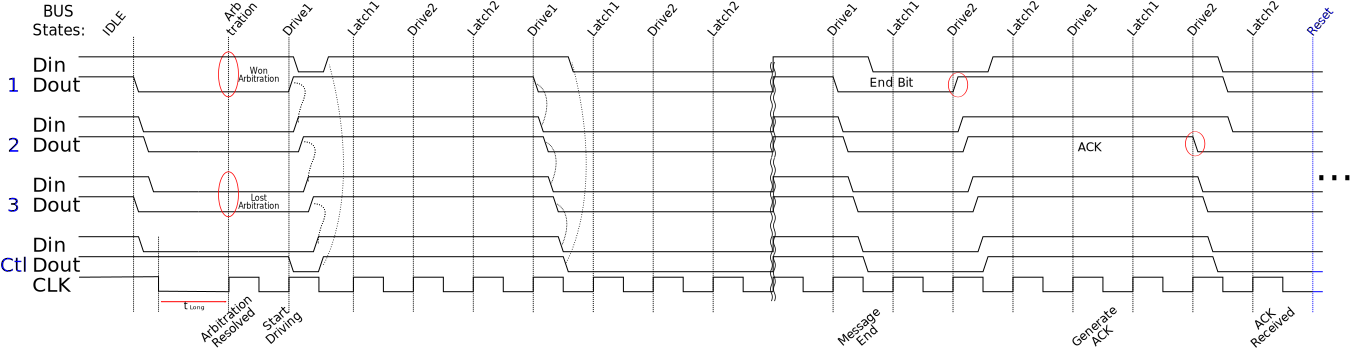
\includegraphics[width=\linewidth]{img/timing}
\caption{A complete transmission. In this system, there are
three member nodes (1, 2, and 3) and a control node. The data loop is connected
Ctl $\rightarrow 1 \rightarrow 2 \rightarrow 3 \rightarrow$ Ctl. This
demonstrates arbitration between member nodes 1 and 3, which node 1 wins. Node
1 then transmits data ({\tt 1,0,\ldots}) to node 2, which ACK's the data.
Reset is elided for space, see Section~\ref{sec:design-reset} for details of
the Reset sequence.
}
\label{fig:transmission}
\end{figure*}

\subsection{Bus~Idle}
\label{sec:protocol-idle}
In \bus Bus~Idle, all lines ({\tt CLK}, {\tt DIN}, {\tt DOUT}) are high.
All member nodes are in forwarding state and the control node is waiting to
begin arbitration.

\subsection{Arbitration}
\label{sec:protocol-arbitration}
To begin arbitration, the bus must be in idle state.

To request to transmit on the bus, a node should pull its {\tt DOUT} line low.
All member nodes remain in forwarding state during arbitration, thus when
their {\tt DIN} line goes low, they are obligated to pull their {\tt DOUT}
line low. The control node, however, does {\bf NOT} pull its {\tt DOUT} line
low in response to its {\tt DIN} line going low. The control node only pulls
its {\tt DOUT} line low when it wishes to transmit on the bus. When the
control node's {\tt DIN} line goes low, it will pull the {\tt CLK} line low
and hold it low for some period $t_{long}$.

By the end of the period $t_{long}$, the effect of the arbitration is
achieved. A member node is in one of three possible states:
\begin{enumerate}
  \item {\tt CLK} low, {\tt DIN} high, {\tt DOUT} high -- Lost arbitration
    (didn't participate)
  \item {\tt CLK} low, {\tt DIN} high, {\tt DOUT} low -- Won arbitration
  \item {\tt CLK} low, {\tt DIN} low, {\tt DOUT} low -- Lost arbitration
    (either lost, or didn't participate)
\end{enumerate}
If the control node wishes to transmit on the bus, all member nodes will be in
the third state. Note this arbitration protocol introduces a {\em
topology-dependent priority}. Firstly, the control node has a greater priority
than any member node as its {\tt DOUT} will propagate around the entire data
loop. The priority of the member nodes is inversely related to their proximity
to the control node in the data loop. That is, the furthest node from the
control node, the node whose {\tt DIN} is connected to the control node's
{\tt DOUT}, has the highest priority of member nodes. The closest node to the
control node, the node whose {\tt DOUT} is connected to the control node's
{\tt DIN}, has the lowest priority.

At the end of $t_{long}$, the control node drives the {\tt CLK} line high. The
arbitration phase ends on this rising edge. Whichever node won the arbitration
transitions from a forwarding node to a transmitting node. If it is not the
transmitting or receiving node, the control node enters forwarding mode for
the duration of the transmission.

The rising edge that established the arbitration winner
is defined as a {\sc latch2} edge. This means the next clock edge will be a
{\sc drive1}, when the transmitting node should send the first bit of the
destination address.

\subsection{Message Transmission}
\label{sec:protocol-transmission}
During transmission, \bus alternates between the {\sc drive1}, {\sc latch1},
{\sc drive2} and {\sc latch2} states on every rising {\tt CLK} edge. 
Note, for forwarding (and receiving) nodes, the {\tt DIN} and {\tt DOUT} lines 
are {\bf NOT} clocked, nodes should forward data signals immediately.

The first rising edge after arbitration starts the first {\sc drive1} state.
After {\tt CLK} goes high, the transmitting node should set its {\tt DOUT}
line to {\tt 0} or {\tt 1} as appropriate. At the next rising edge, \bus
switches to {\sc latch1} state and nodes latch the value on their {\tt DIN}
lines. The next rising edge starts the {\sc drive2} state. During {\sc drive2}
the transmitting node should \textbf{forward} its {\tt DIN} value as opposed
to driving the data bit again. During a normal
transmission, the value forwarded will not change, but if any node desires to
reset the bus, they may do so by setting the opposite bit during {\sc drive2},
initiating a Bus~Reset event\footnote{
  Caution must be taken by a resetting node to not introduce a false
  Message~End~Sequence. See the note in~\ref{sec:protocol-reset} for details.}
The final state is {\sc latch2} at the next rising edge, where the same bit is
read again, matching the bit read during {\sc latch1}.  It is at this
point---when the same bit has been received during {\sc latch1} and {\sc
latch2}---that the receiving layer records the incoming bit. The next clock
edge starts the sequence over, returning to {\sc drive1}.

The first sequence of bits pushed onto \bus are the {\em address} bits. All
nodes on a \bus should listen until their address:
\begin{itemize}
  \item Matches: Node promotes itself from forwarder to receiver.
  \item Does Not Match: Node remains forwarder for the rest of the
    transmission.
\end{itemize}

There is no protocol-level delineation between address and data bits. The
transmitting node sends address$+$data as a continuous stream of bits until
it terminates the message with a Message~End~Sequence.

\hl{TODO:} The \bus addressing scheme has not yet been defined.

\subsection{Message End Sequence}
\label{sec:protocol-end}
Picking up transmission from the last bit of data the transmitting node wishes
to send, the transmitting node pushes its last bit on its {\tt DOUT} line
during the {\sc drive1} state, and it is latched by \bus during the {\sc
latch1} and {\sc latch2} states.  At the next {\sc drive1} state, the 
transmitting node drives its {\tt DOUT} line low. This low half-bit is a sentinel 
stop bit---it is not part of the transmitted message, rather the beginning of 
the Message~End~Sequence. At the rising edge of the {\tt CLK} that starts the
{\sc latch1} state, all \bus nodes latch {\tt 0}. The next rising edge of the
{\tt CLK}, which starts {\sc drive2} state, the transmitting node drives its 
{\tt DOUT} line high. At the next rising {\tt CLK} edge, which starts the next 
{\sc latch2} state, nodes will observe that the data line differs from 
{\sc latch1} state. The receiving and control nodes will recognize this
{\tt 01} sequence as a Message~End~Sequence.

At the next rising edge after transmitting the stop sequence, the transmitting
node should begin forwarding its {\tt DIN} to its {\tt DOUT} and listening for
an acknowledgement.

\subsection{Message Acknowledgement}
\label{sec:protocol-ack}
After the Message~End~Sequence, the receiving layer is responsible for sending a
Message Acknowledgement. The receiver cannot detect the Message~End~Sequence
until the {\sc latch2} that ended the previous cycle.

At the next rising clock edge, a {\sc drive1}, the receiving layer continues
to forward {\tt DIN} to {\tt DOUT}, which functionally drives a {\tt 1} as the
data ring should already be high from the end of the Message~End~Sequence. The
value {\tt 1} is latched by \bus at the next clock edge during {\sc latch1}.
At the next clock edge, {\sc drive2}, the receiving layer should drive {\tt 0}
if it wishes to acknowledge the transmission. The acknowledgement is confirmed
at the next clock edge, {\sc latch2}.

This is a relatively fast turnaround for the receiving node. It has from {\sc
latch2} when it detects the Message~End~Sequence until the next {\sc drive2} to
determine whether or not it wishes to acknowledge the transmission. Designers
should take care to ensure the acknowledge signal logic can be generated in
half a bit time (2 clock pluses).


\subsection{Bus Reset}
\label{sec:protocol-reset}
The \bus Reset is designed to be particularly robust. For details on Reset
design decisions, see~\ref{sec:design-reset}~\nameref{sec:design-reset}. Here
we describe Reset functionally.

A Bus Reset can only be performed by the control node. Member nodes can
request that the control node reset the bus by generating illegal signals such
as transitions during {\sc latch} cycles are a {\tt 10} sequence any time
except Acknowledgement.

During reset, the control node halves the speed of the \bus~{\tt CLK} line.
The controller's internal clock is still running at full speed. The control
layer uses these extra edges to reliably drive values onto the data lines in
the face of unreliable nodes, see Figure~\ref{fig:reset-normal} for details of
the timing of the extra edges.

The control node begins reset by driving {\tt 0}. It alternates between
driving {\tt 0} and {\tt 1} until its {\tt DIN} history buffer contains the
sequence {\tt 010}. For any member node, latching the sequence {\tt 010} {\em
unconditionally} transitions the node to {\sc reset}. The robustness of this
detection is paramount. The recommended practice is a small 3-bit shift
register that records every latched bit. If the pattern {\tt 010} ever appears
in this register, a signal should be asserted that directly moves the node
into {\sc reset}, conceptually:

\begin{quote}
\lstset{
  language=Verilog,
  basicstyle=\ttfamily,
  keywordstyle=\color{OliveGreen}\textbf,
  literate={`}{{\`{}}}1 {'}{{\'{}}}1
}
\begin{lstlisting}
wire reset_history = (reset_history_reg == 3'b010);

always @(posedge clock) begin
  state <= (reset_history) ? `STATE_RESET : next_state;
\end{lstlisting}
\end{quote}

As the only clock driving state machines in \bus is the \bus~{\tt CLK} line,
an edge is required to actually push the state machine into {\sc reset} after
detecting the need in {\sc latch1/2}. We call this edge Phase-Align for reasons
exaplined in~\ref{sec:design-reset-phase}~\nameref{sec:design-reset-phase} and
continue to hold data low during this cycle. After the Phase-Align edge,
member nodes sample on {\em every} edge.

Finally, the control node drives the data line high and drives two cycles. The
{\tt 11} (or possibly {\tt 011} if a node is $1\phi$ or $3\phi$) marks the
completion of reset. The final clock edge finishes the transaction, returning
\bus to Idle.

If a node records a sequence other than {\tt 11} or {\tt 011} during Reset, an
error has occurred. If the node is simply forwarding, it should return to
forwarding and await the real Reset so as to avoid needlessly interrupting an
otherwise succeeding transmission. If the node was transmitting or receiving
it should enter into {\sc error} to abort the current transaction as it is no
longer salvageable.

More details and subtleties of Reset are covered
in~\ref{sec:design-reset}~\nameref{sec:design-reset}.
